\begin{frame}{Variational Quantum Algorithms (VQAs) in the Wild}
  \vspace*{-3mm}
  \begin{figure}
      \captionsetup{justification=centering}
      \begin{minipage}{.5\textwidth}
        \caption*{\textbf{Utility Before Fault Tolerance} \\ (Nature 618, 500–505)}
          \vspace*{-3mm}
          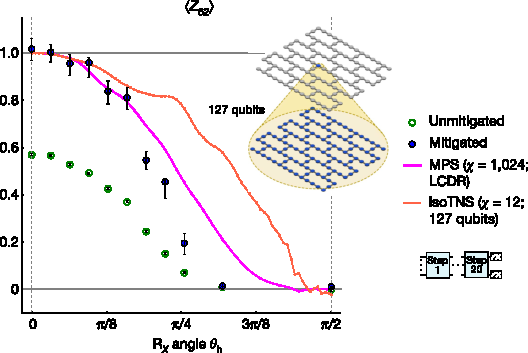
\includegraphics[height=0.35\textheight, center]{evidence_of_utility_before_fault_tolerence.pdf}
      \end{minipage}%
      \begin{minipage}{0.5\textwidth}
        \caption*{\textbf{Quantum Many-body Dynamics} (arXiv:2307.07552)}
          \vspace*{-3mm}
          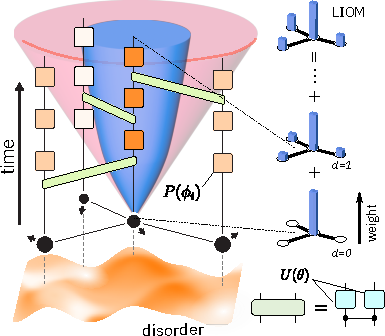
\includegraphics[height=0.35\textheight, center]{quantum_many_body_dynamics.pdf}
      \end{minipage}
  \end{figure}%
  \vspace*{-2mm}
  \begin{figure}

      \captionsetup{justification=centering}
      \begin{minipage}{.5\textwidth}
        \caption*{\textbf{Quantum Spin Chains} (arXiv:2207.0999)}
          \vspace*{-3mm}
          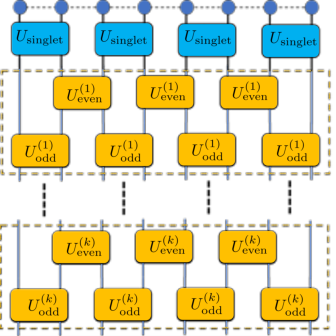
\includegraphics[height=0.35\textheight, center]{large_size_quantum_spin_chains.pdf}
      \end{minipage}%
      \begin{minipage}{0.5\textwidth}
        \caption*{\textbf{Nishimori transition} (arXiv:2309.02863)}
          \vspace*{-3mm}
          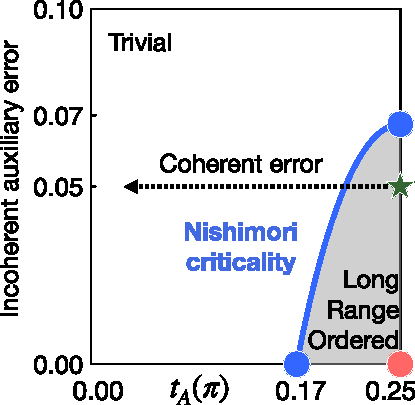
\includegraphics[height=0.35\textheight, center]{nishimori_transition.pdf}
      \end{minipage}
  \end{figure}
\end{frame}

\begin{frame}{Variational Quantum Algorithms (VQAs)}
   \vspace*{-4mm}
   \begin{figure}
      \centering
      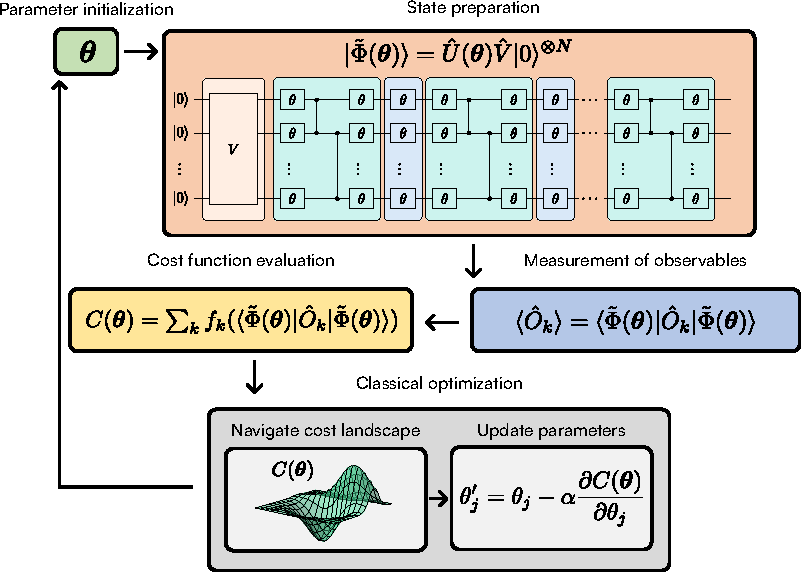
\includegraphics[height=0.89\textheight]{vqa_schematic.pdf}
    \end{figure}
\end{frame}


\begin{frame}{Cost Landscapes in Variational Quantum Algorithms}
 \vspace{-5mm}
 \begin{columns}
    \begin{column}{0.5\linewidth}
      \begin{itemize}
        \item[(a)] Clear separation of cost function values.
        \item[(b)] Concentration of cost function values.
        \item[(c)] Recovery of features keys of noiseless cost function values.
      \end{itemize}
    \end{column}%
    \begin{column}{0.5\linewidth}
       \begin{figure}
          \centering
          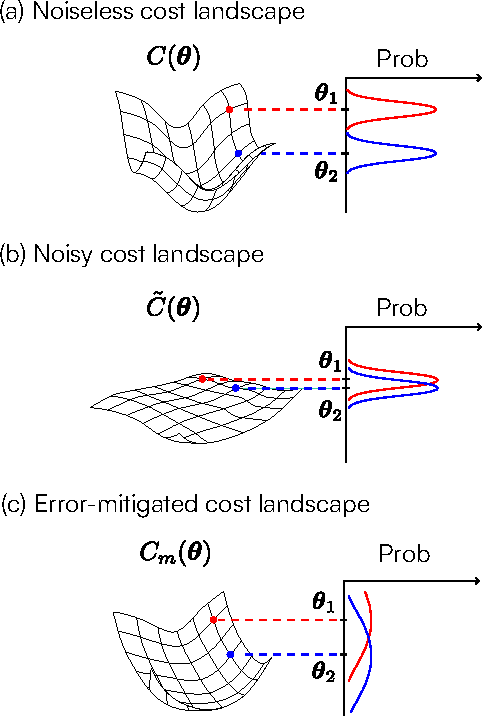
\includegraphics[height=0.80\textheight]{vqa_landscapes.pdf}
          \caption*{arXiv:2109.0105}
        \end{figure}
    \end{column}

  \end{columns}
\end{frame}


\begin{frame}{Hyperparameter Tuning}
   \vspace*{-4mm}
   \begin{figure}
      \centering
      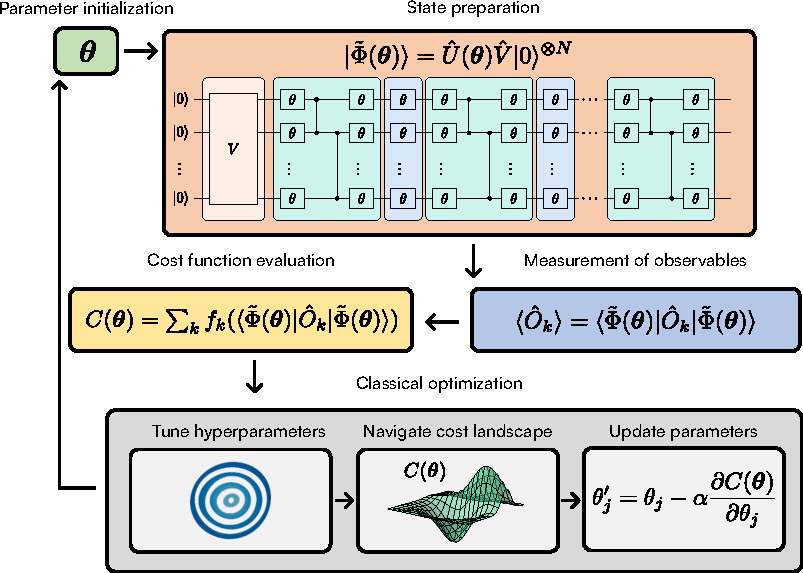
\includegraphics[height=0.89\textheight]{vqa_optuna_schematic.pdf}
    \end{figure}
\end{frame}
